% Drawing 148/02-11 -- folder 148, batch 02, archive page 31 (PDF page 32).
% Transcription: au crayon, sans texte : une sphère avec son équateur portant deux points, un troisième point au-dessus ; à droite, une bipyramide à base quadrilatère dont les sommets sont marqués ; plus à droite, un ovale à peine visible.
% Kind: pencil sphere with equator; bipyramid with marked vertices. Method 2 (schematic redraw from the facsimile). Status: ok.
% Notes: Very faint pencil on the back of a listing (seen with the contrast raised). Left: a sphere outline (doubled at its sides, drawn once), its equator as a flat ellipse with two points on it and one point above it inside the outline. Middle: a bipyramid: a top vertex, the four vertices of a quadrilateral base and a bottom vertex at the edge of the typed lines; the base drawn as a closed quadrilateral, the top joined to the four base vertices, the bottom joined to the four base vertices (the stroke from the left base vertex doubled), one more short stroke between the right base vertex and the bottom; a curved stroke rising from the top vertex. Right: two long faint strokes that converge downwards from the top of the crop, a stroke from the first of them to the right, a short stroke at their foot, and an open oval drawn twice round a point. Left out: the typed lines of the listing. Redrawn 2026-11-12 (issue 128). 2026-11-13, Claude Opus 5.5, issue 147, overlay check: not compiled (no TeX in the session); the TikZ was rasterised by a local interpreter and laid over the 403 ppi scan rendered at 400 dpi, contrast raised. Redrawn on the ink: vertices and points on the centres of their blots, straight strokes fitted on their ink, curves through points moved onto their ink; every stroke lies on its ink to within about one unit (the faintest pencil within its own width). Changed: the vertices of the bipyramid and the sphere moved onto the page (they were up to four units off); the bottom vertex is at the foot of the figure, not in the middle; the curved stroke from the top vertex, the doubled stroke to the bottom, and the strokes and second oval at the right are now drawn. The transcription's « un ovale à peine visible » is these strokes and the doubled open oval.
% Coordinates: 1 unit = 1 mm = 1/100 of the crop width, y downwards as on the crop (bbox in page fractions: [0.44, 0.13, 0.94, 0.33]).
% Redrawn by Claude (claude-fable-5-2), issue #128, 2026-11-12; not checked by a human; not compiled (no TeX in the session); overlay-checked on the scan by Claude Opus 5.5, issue #147, 2026-11-13, not compiled (no TeX in the session).
% Rights: reproduces part of the work -- behind RENDER_TRANSCRIPTS, never published by itself.
\documentclass[tikz,border=3pt]{standalone}
\usepackage{amsmath,amssymb}
\usetikzlibrary{patterns,arrows.meta}
\tikzset{pencil/.style={black!45}, struck/.style={black!35}, mpt/.style={circle,draw,inner sep=1.3pt}, pt/.style={circle,fill,inner sep=0.9pt}, opt/.style={circle,draw,fill=white,inner sep=1.1pt}, Rd/.style={red!75!black}, Gn/.style={green!45!black}, Br/.style={brown!70!black}}
\begin{document}
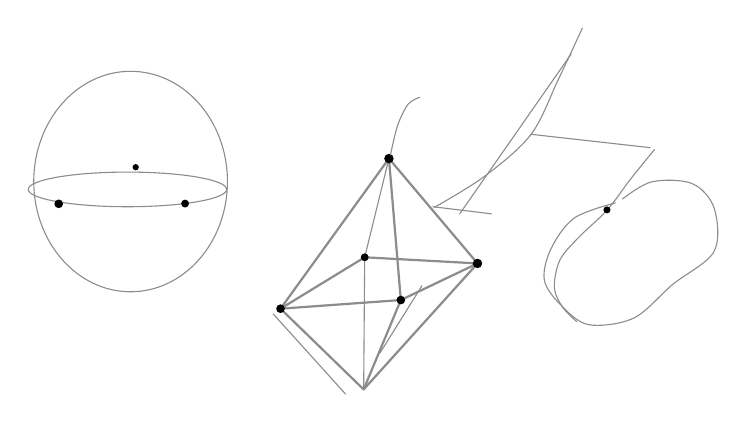
\begin{tikzpicture}[x=1mm,y=-1mm,line cap=round,line join=round,font=\small]
% sphere: outline (doubled at its sides on the page, drawn once), equator, two points on it and one above it
\draw[pencil] (22.8,21.5) ellipse [x radius=12.3, y radius=14];
\draw[pencil] (22.4,22.5) ellipse [x radius=12.6, y radius=2.2];
\fill (13.67,24.33) circle [radius=0.55];
\fill (29.72,24.3) circle [radius=0.5];
\fill (23.45,19.68) circle [radius=0.4];
% bipyramid: top vertex, four vertices of the quadrilateral base, bottom vertex (at the edge of the typed lines)
\coordinate (T) at (55.61,18.58);
\coordinate (a) at (41.84,37.65);
\coordinate (b) at (52.53,31.12);
\coordinate (c) at (66.86,31.9);
\coordinate (d) at (57.12,36.55);
\coordinate (B) at (52.4,47.9);
\draw[pencil,thick] (a) -- (b) -- (c) -- (d) -- cycle;
\draw[pencil,thick] (T) -- (a);
\draw[pencil] (T) -- (b);
\draw[pencil,thick] (T) -- (c);
\draw[pencil,thick] (T) -- (d);
\draw[pencil,thick] (a) -- (B);
\draw[pencil] (40.91,38.31) -- (50.09,48.48);
\draw[pencil] (b) -- (B);
\draw[pencil,thick] (d) -- (B);
\draw[pencil,thick] (c) -- (B);
\draw[pencil] (59.8,34.74) -- (54.47,43.28);
\fill (T) circle [radius=0.6];
\fill (a) circle [radius=0.55];
\fill (b) circle [radius=0.5];
\fill (c) circle [radius=0.6];
\fill (d) circle [radius=0.55];
% curved stroke rising from the top vertex
\draw[pencil] plot[smooth, tension=0.55] coordinates {(55.81,18.08) (56.72,14.36) (58.04,11.69) (59.51,10.8)};
% at the right: two long faint strokes converging downwards, a stroke from the first to the right, a short stroke at the foot, and an open oval drawn twice round a point
\draw[pencil] plot[smooth, tension=0.55] coordinates {(80.17,2.03) (77.11,8.56) (73.65,15.52) (67.76,20.83) (61.38,24.78)};
\draw[pencil] (78.75,5.31) -- (64.6,25.6);
\draw[pencil] (73.65,15.5) -- (88.8,17.2);
\draw[pencil] (61.2,24.7) -- (68.6,25.6);
\draw[pencil] plot[smooth, tension=0.55] coordinates {(84.35,24.21) (79.12,26.15) (76.17,30.08) (75.34,33.98) (77.35,37.09) (80.94,39.67) (86.7,38.84) (91.63,34.58) (96.89,30.4) (96.92,24.9) (94.12,21.76) (89.01,21.53) (85.28,23.71)};
\draw[pencil] plot[smooth, tension=0.55] coordinates {(89.32,17.45) (86.28,21.21) (83.33,25.11) (79.66,28.64) (77.31,31.5) (76.62,35) (77.66,37.44) (79.47,39.3)};
\fill (83.3,25.1) circle [radius=0.45];
\end{tikzpicture}
\end{document}
